\documentclass[border=10pt]{standalone}
\usepackage{tikz}\usepackage{amsmath}\usetikzlibrary{calc,arrows.meta}
\begin{document}
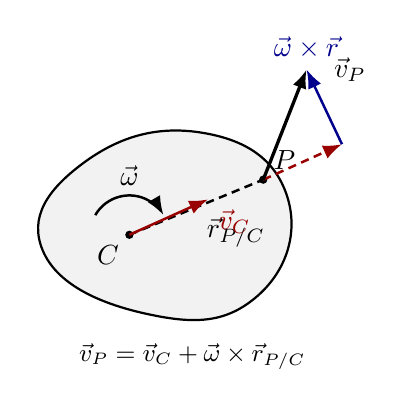
\begin{tikzpicture}[line width=0.9pt,>={Latex[length=2.4mm]}]
  \draw[thick,fill=black!5] plot[smooth cycle,tension=0.8] coordinates {(-0.2,1.1)(1.3,1.5)(2.4,0.7)(2.0,-0.6)(0.6,-0.8)(-0.7,0.0)};
  \coordinate (C) at (0.4,0.2); \coordinate (P) at (2.1,0.9);
  \fill (C) circle(1.5pt) node[below left]{$C$};
  \fill (P) circle(1.5pt) node[above right]{$P$};
  \draw[densely dashed] (C)--(P) node[midway,below right]{$\vec r_{P/C}$};
  % omega en C
  \draw[->] ($(C)+(150:0.5)$) arc (150:30:0.5); \node at ($(C)+(0.0,0.75)$){$\vec\omega$};
  % traslacion v_C (mismo en C y P)
  \draw[->,red!60!black] (C)--($(C)+(1.0,0.45)$) node[below right]{$\vec v_C$};
  \draw[->,red!60!black,densely dashed] (P)--($(P)+(1.0,0.45)$);
  % rotacion: omega x r (perp a r)
  \draw[->,blue!55!black] ($(P)+(1.0,0.45)$)--($(P)+(0.55,1.4)$) node[above]{$\vec\omega\times\vec r$};
  % resultante
  \draw[->,line width=1.2pt] (P)--($(P)+(0.55,1.4)$) node[right=6pt]{$\vec v_P$};
  \node at (1.2,-1.35){\small $\vec v_P=\vec v_C+\vec\omega\times\vec r_{P/C}$};
\end{tikzpicture}
\end{document}
